\chapter{Diseño de Software}

\paragraph{}
Se optó por utilizar una arquitectura Time-Triggered cooperativa, donde
las tareas se corresponden con los subsistemas de Hardware:

\begin{itemize}
	\item
	Control de motores
	\item
	Recepción inalámbrica
	\item
	Detector de obstáculos
\end{itemize}

Además de la interrupción de tiempo, propia de la arquitectura Time
Triggered, se necesita una interrupción de tiempo independiente
utilizada por el sensor de proximidad para medir con presición la
distancia a la que se encuentran los obstáctulos.

El psuedocódigo del programa principal se resume a lo siguiente:

\begin{Verbatim}
interrupcion 50ms:
	flag_tiempo = 1

variables compartidas:
	accion_vehiculo # Enumerativo que indica el desplazamiento que
			# se debe realizar


programa principal:
	inicializacion motores
	inicializacion bluetooth
	inicializacion detector de colisiones
	prender led power

super loop:
	si flag_tiempo = 1:
		leer bluetooth
		detectar colisiones
		actualizar motores
		flag_tiempo = 0
\end{Verbatim}


\section{Pseudocódigo de los Módulos}

\subsection{Leer Bluetooth}

\begin{Verbatim}
si hay mensajes nuevos:
	leer el mensaje
	si es una A o a:
		motor = avance
	si es una C o C:
		motor = retrocede
	si es una D o d:
		motor = giro izquierda
	si es una B o b:
		motor = giro derecha
	si es un 0:
		motor = giro libre
	si es una F o f:
		motor = freno
\end{Verbatim}

\subsection{Detectar Colisiones}

\paragraph{}El eco producido por el módulo se genera -aproximadamente- entre 60uS y
12mS. Creemos que no es necesario realizar las mediciones cada estos
periodos tan cortos de tiempo, dado que, puede ser contraproducente para
los tiempos del sistema considerando el objetivo del sensor. Por esto,
el procesamiento del se realiza cada 250ms:

\begin{Verbatim}
inicializar detector de colisiones:
	tick_colision = 0

detectar colisiones:
	tick_colision++
	si tick_colision = 5:
		tick_colision = 0
		tomar tiempo
		prender input capture
		enviar señal de comienzo de medicion

si llego el echo:
	calcular distancia
	si hay un obstaculo cerca:
		bloquear movimiento hacia adelante
\end{Verbatim}

\subsection{Actualizar Motores}

\paragraph{} Los motores se controlan en dos niveles: a bajo nivel se puede controlar cada
motor de manera independiente, indicando la dirección de giro. Una capa
más ``alta'' permite controlar el vehículo más facilmente, brindando
funciones para indicar como se debe mover el vehículo.

\begin{figure}[H]
	\centering
	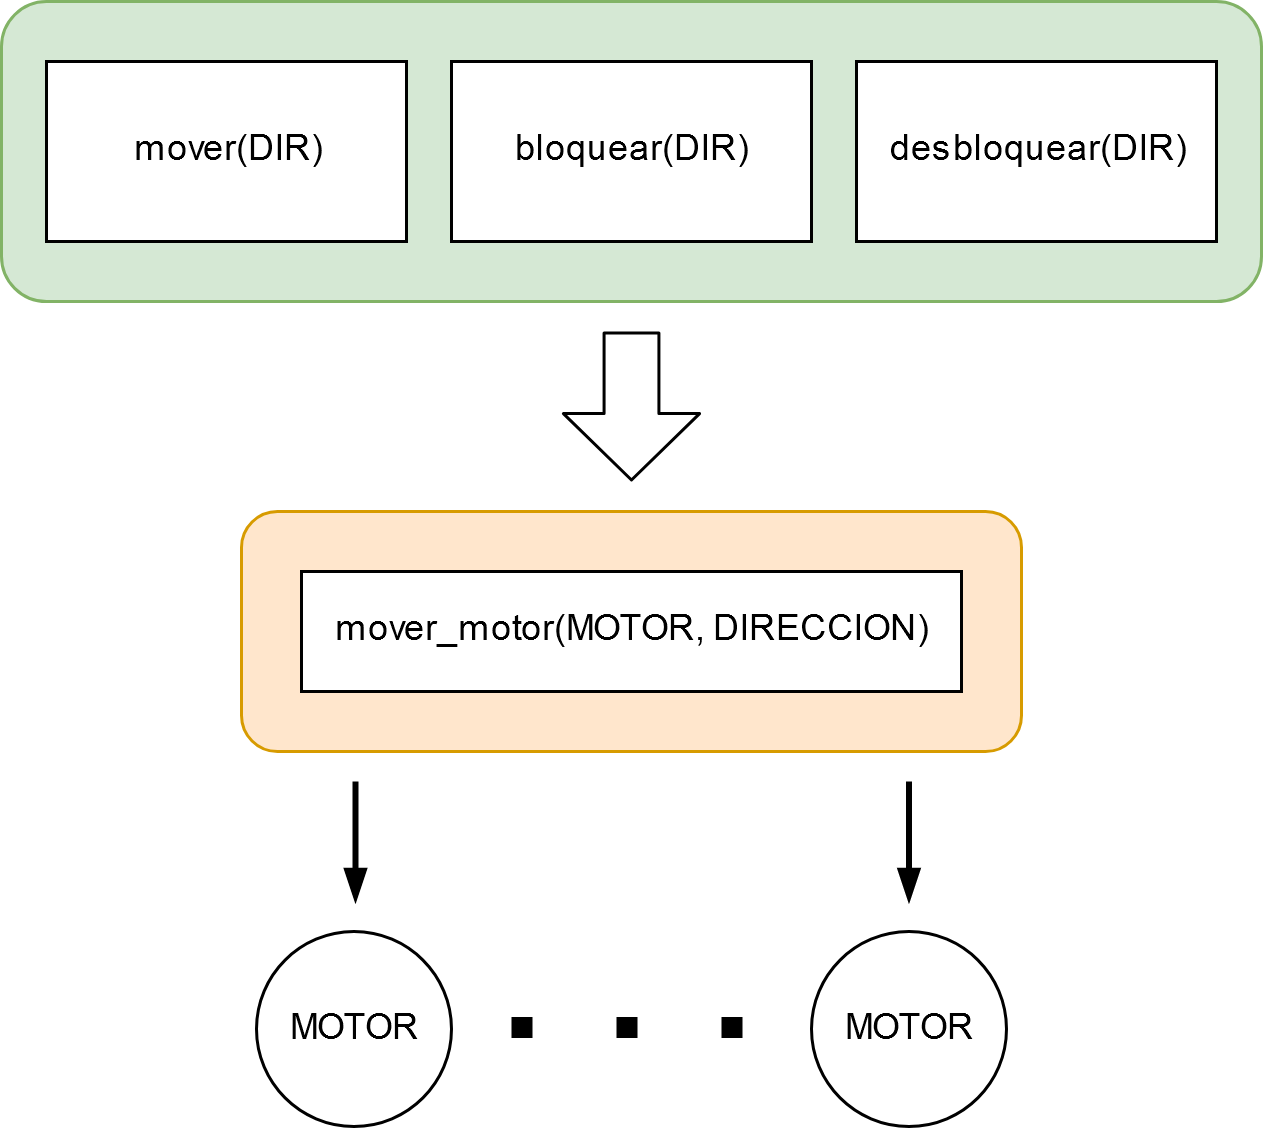
\includegraphics[width=0.5\linewidth]{informe_2/capas_motor}
	\caption{Capas de los Motores}
	\label{fig:capasmotor}
\end{figure}


Por lo que el pseudocódigo se reduce a lo siguiente

\begin{Verbatim}
inicializacion de motores:
	setear movimiento en libre

actualizacion de motores:
	ver accion_vehiculo
	mover el vehiculo en la direccion solicitada

	# A modo de ejemplo se explica como mover en una sola direccion
	si movimiento es hacia adelante:
		motor trasero izquierdo girar horario
		motor trasero derecho girar antihorario
		motor delantero izquierdo girar horario
		motor delantero derecho girar horario
	...
\end{Verbatim}

A bajo nivel se controla cada motor individualmente:

\begin{Verbatim}
si movimiento es horario:
	colocar canal 1 en alto
	colocar canal 0 en bajo
si movimiento es anti horario:
	colocar canal 0 en bajo
	colocar canal 1 en alto
\end{Verbatim}

\subsection{Software Android}

\paragraph{BLEJoystick}
BLEJoystick es la aplicación a utilizar para el control inalámbrico del
vehículo, está disponible para múltiples dispositivos android y se puede
descargar de manera gratuita desde Google Play Store. Esta aplicación se
conecta al módulo bluetooth HM-10 mediante el protocolo bluetooth low
energy 4.0 (BLE). Cuenta con 8 botones, donde el funcionamiento de cada
uno es el siguiente: 

\begin{itemize}
	\item
	Cuando se presiona por primera vez, envía una letra en mayúscula.
	\item
	Mientras siga presionado el mismo botón, envía la misma letra en
	minúscula de manera constante.
	\item
	Cuando se suelta el boton, envía un 0.
\end{itemize}

A continuación se describe cada uno de los botones y su letra
correspondiente:

\begin{longtable}[]{@{}lll@{}}
	\toprule
	Botón & Letra inicial & Letra constante\tabularnewline
	\midrule
	\endhead
	Arriba & A & a\tabularnewline
	Derecha & B & b\tabularnewline
	Abajo & C & c\tabularnewline
	Izquierda & D & d\tabularnewline
	Triángulo & E & e\tabularnewline
	Círculo & F & f\tabularnewline
	Equis & G & g\tabularnewline
	Cuadrado & H & h\tabularnewline
	\bottomrule
\end{longtable}

\section{Interfaz de Usuario}

\subsection{Pasos a seguir para la configuración del sistema}

\begin{figure}[H]
	\centering
	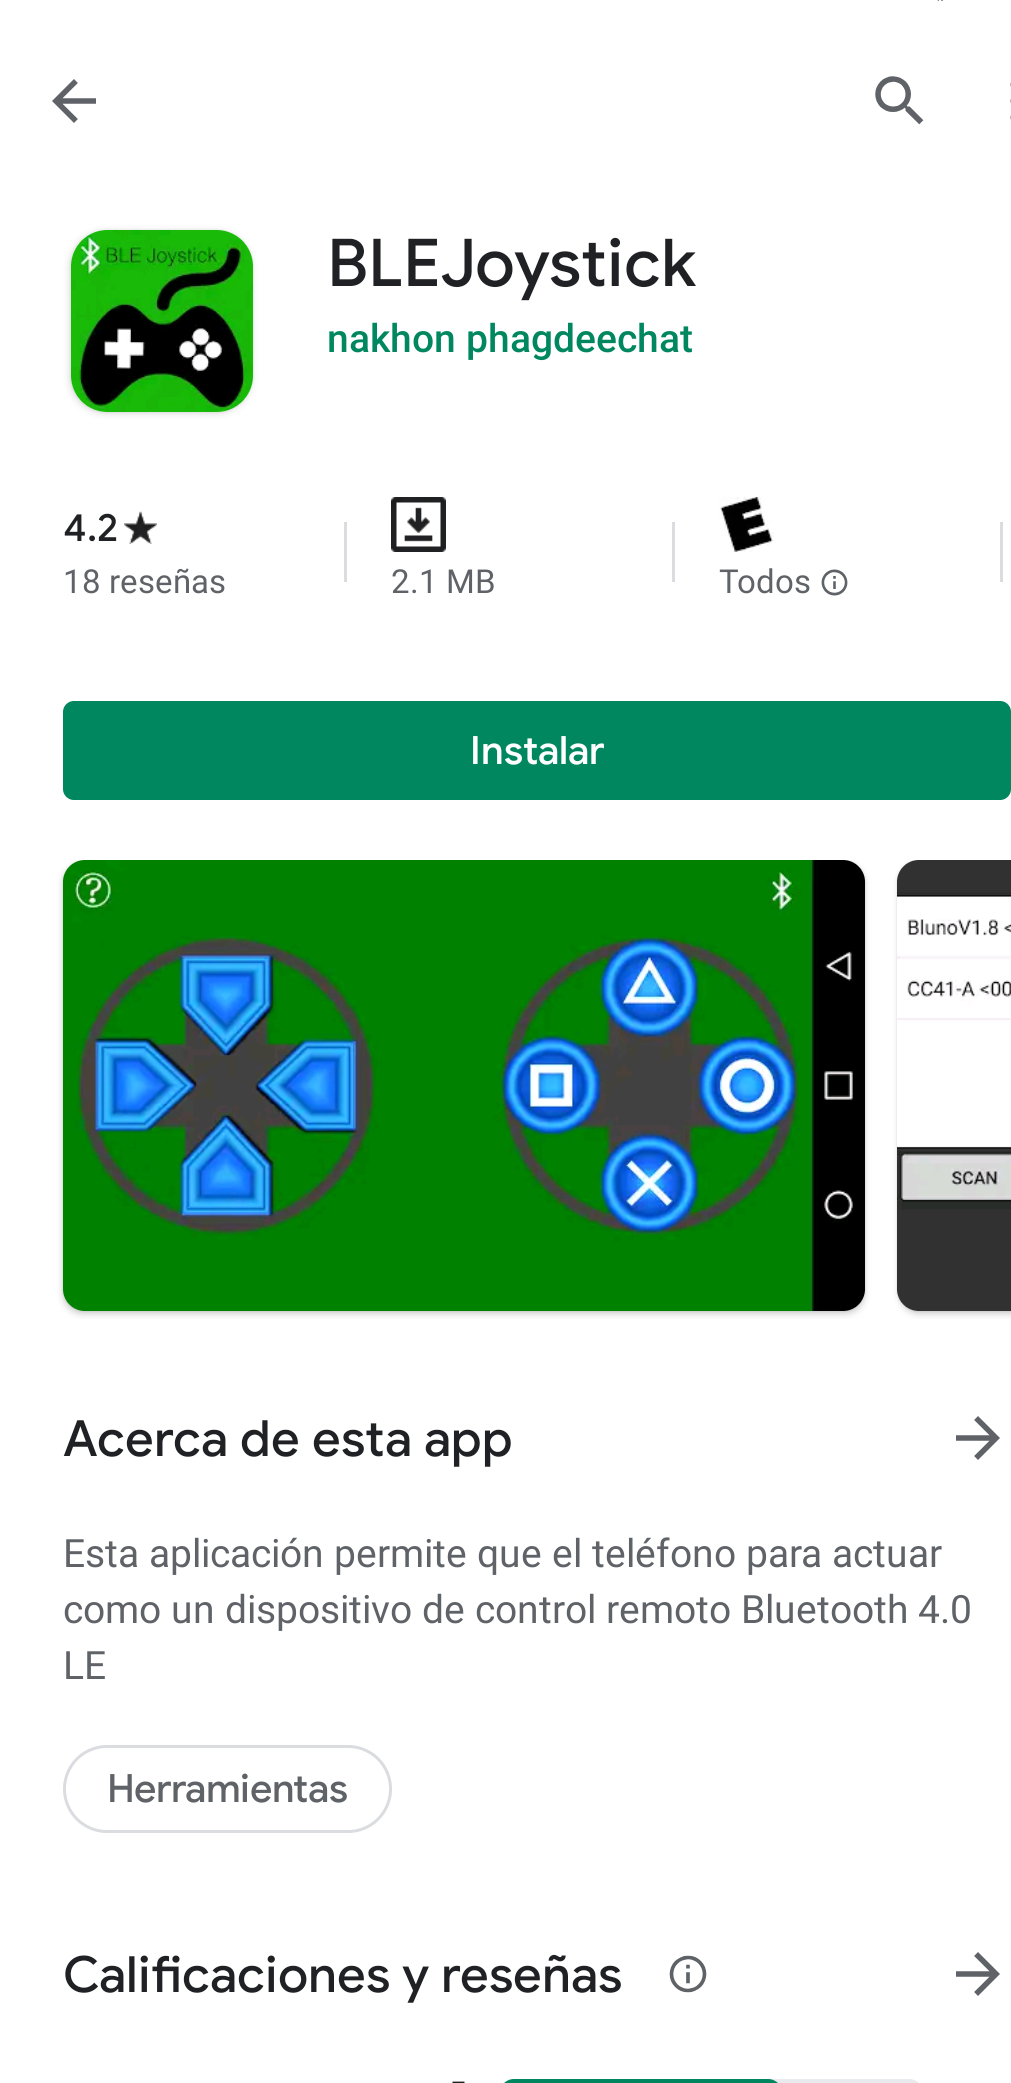
\includegraphics[width=0.5\linewidth]{informe_2/interfaz_joystick_store}
	\caption{Aplicación en el Play Store}
	\label{fig:interfazjoystickstore}
\end{figure}

\begin{enumerate}
	\def\labelenumi{\arabic{enumi}.}
	\item
	Ingresar a Google Play Store
	\item
	Descargar la aplicación BLEJoystick
	\item
	Iniciar la aplicación.
	\item
	Pulsar el ícono de vinculación bluetooth y seleccionar
	\emph{vehiculo}.
	\item
	Corroborar la correcta vinculación mediante el LED indicador.
	\item
	Sistema listo para usar.
\end{enumerate}

\subsection{Utilización del Vehículo}

\begin{figure}[H]
	\centering
	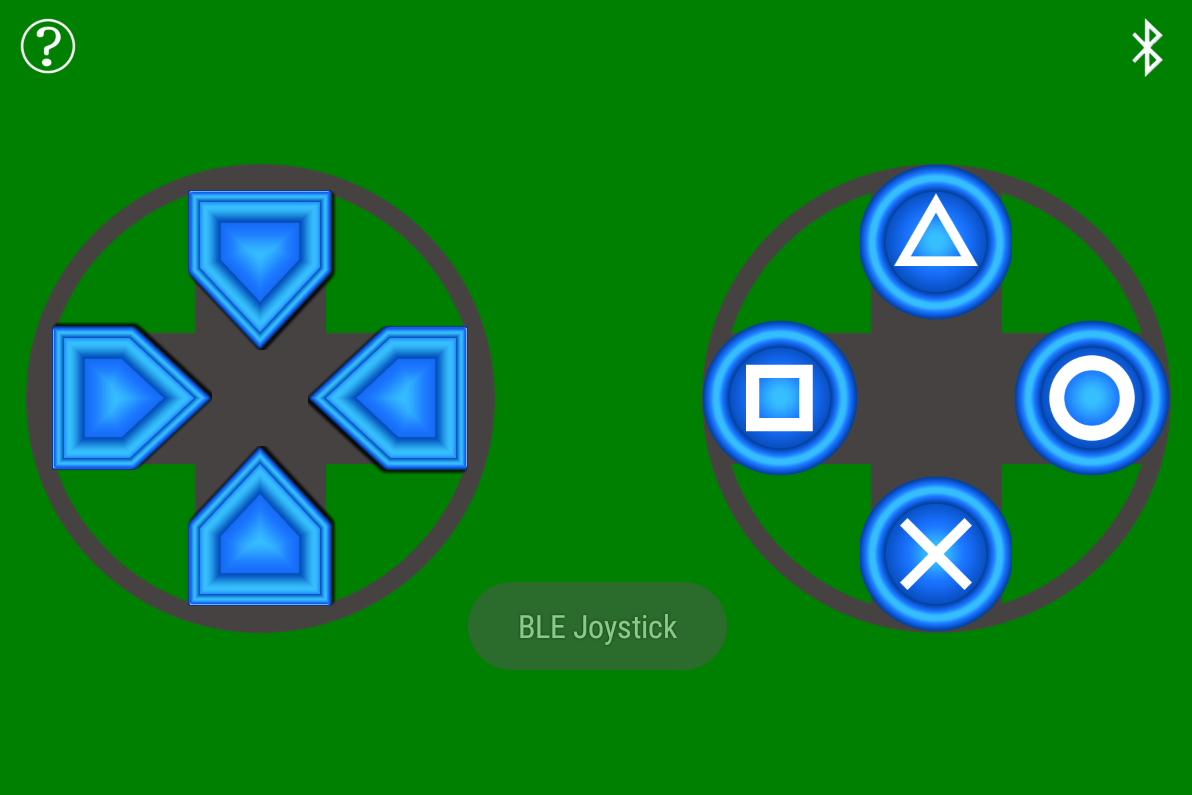
\includegraphics[width=0.7\linewidth]{informe_2/interfaz_joystick}
	\caption{La aplicación BLEJoystick}
	\label{fig:interfazjoystick}
\end{figure}

A continuación se detalla y explica el funcionamiento 
de cada uno de los botones disponibles en la aplicación
\begin{longtable}[]{@{}ll@{}}
	\toprule
	Botón & Función\tabularnewline
	\midrule
	\endhead
	Arriba & Desplazar hacia adelante\tabularnewline
	Derecha & Girar hacia la derecha\tabularnewline
	Abajo & Desplazar hacia abajo\tabularnewline
	Izquierda & Girar hacia la izquierda\tabularnewline
	Círculo & Frenar\tabularnewline
	\bottomrule
\end{longtable}

\section{Librerías de Software}

\paragraph{sAPI} Dada la extensión de la librería provista por la CIAA, solo se requiere
usar esta. Más específicamente se utilizaran las librerías
\texttt{sapi\_pwm.h}, \texttt{sapi\_gpio.h}
y \texttt{sapi\_timer.h}.

\section{Ensayos}

\subsection{Motores y L293D}

\paragraph{}Realizamos una prueba de los motores con los L293D, para esto realizamos un prototipo de la estructura del vehículo con el objetivo de observar el correcto funcionamiento tanto de los motores como del chip L293D y verificar si la potencia de los motores será suficiente para mover el vehículo con todos sus componentes a una velocidad considerable. 

El ensayo se realizó con una placa de Arduino con un shield para controlar motores, donde todos los motores fueron configurados con la máxima velocidad posible, generando el siguiente el código de prueba:

\begin{lstlisting}[language=C,basicstyle=\footnotesize\ttfamily]

#include <AFMotor.h>

AF_DCMotor motor1(1);	// Declara los motores a utilizar
AF_DCMotor motor2(2);
AF_DCMotor motor3(3);
AF_DCMotor motor4(4);

void setup() {
	Serial.begin(9600);	// Inicializa la terminal serie a 
						// 9600 bps
	Serial.println("Prueba de motores");


	motor1.run(RELEASE);	// Desbloquea el motor
	motor1.run(FORWARD);    // Mueve para adelante
	motor1.setSpeed(255);   // Velocidad entre 0 y 255,
                            // configurada al maximo
	
	motor2.run(RELEASE);
	motor2.run(FORWARD);
	motor2.setSpeed(255);
	
	motor3.run(RELEASE);
	motor3.run(FORWARD);
	motor3.setSpeed(255);
	
	motor4.run(RELEASE);
	motor4.run(FORWARD);
	motor4.setSpeed(255);
}

void loop() {
}
\end{lstlisting}

\paragraph{Conclusiones} Los motores son lo suficientemente potentes como para mover el vehículo a una velocidad considerable, siempre y cuando los L293D sean alimentados con aproximadamente 8V, ya que hay una diferencia entre la entrada del L293D y la salida a cada uno de los motores de ~=2V (los motores van a su máxima velocidad con 6V).

\subsection{PWM}

\paragraph{} Para el análisis preliminar de PWM, se utilizó como código de prueba el ejemplo \verb|pwm_dimmer|. Dicho código utiliza la modulación de ancho de pulso para variar la intensidad de los LEDs alojados en la placa de la EDU CIAA.  A partir de dicho análisis se determinó la necesidad de configurar las correspondencias entre los canales del SCT con los pines del microcontrolador, ya que el proyecto requiere un total de 8 salidas PWM y con la configuración por defecto no eran suficientes; los canales asociados a  CTOUT2, CTOUT4 y CTOUT5 están vinculados a los pines P2\_10, P2\_11 y P\_12 correspondientes a los leds de la placa, dicha relación se establece en el archivo \verb|sapi\_sct.c| ubicado en las librerías del firmware v3 correspondientes a la sAPI. La modificación requerida consiste en derivar la salida del CTOUT2 a LCD1 de la siguiente manera:

\begin{lstlisting}[language=c,basicstyle=\footnotesize\ttfamily]
static pinInitLpc4337_t SCTdataList[] = {

// Configuracion por default:
...
/* Sct n | port | pin | name in board */
/* CTOUT2 */ { 4 , 10 }, /* LED1 */
...

// Configuracion requerida:
...
/* Sct n | port | pin | name in board */
/* CTOUT2 */ { 4 , 4 }, /* LCD1 */
...

}
\end{lstlisting}

Finalmente se verificó el correcto funcionamiento corriendo el programa y conectando en el terminal 30 de la placa, indicado como LCD1, un LED con su correspondiente resistencia.